\documentclass[12pt, oneside]{article}

\usepackage[letterpaper, scale=0.89, centering]{geometry}
\usepackage{fancyhdr}
\setlength{\parindent}{0em}
\setlength{\parskip}{1em}

\usepackage{tikz}
\usetikzlibrary{automata,positioning,arrows}

\pagestyle{fancy}
\fancyhf{}
\renewcommand{\headrulewidth}{0pt}
\rfoot{\href{https://creativecommons.org/licenses/by-nc-sa/2.0/}{CC BY-NC-SA 2.0} Version \today~(\thepage)}

\usepackage{amssymb,amsmath,pifont,amsfonts,comment,enumerate,enumitem}
\usepackage{currfile,xstring,hyperref,tabularx,graphicx,wasysym}
\usepackage[labelformat=empty]{caption}
\usepackage{xcolor}
\usepackage{multicol,multirow,array,listings,tabularx,lastpage,textcomp,booktabs}

\lstnewenvironment{algorithm}[1][] {   
    \lstset{ mathescape=true,
        frame=tB,
        numbers=left, 
        numberstyle=\tiny,
        basicstyle=\rmfamily\scriptsize, 
        keywordstyle=\color{black}\bfseries,
        keywords={,procedure, div, for, to, input, output, return, datatype, function, in, if, else, foreach, while, begin, end, }
        numbers=left,
        xleftmargin=.04\textwidth,
        #1
    }
}
{}

\newcommand\abs[1]{\lvert~#1~\rvert}
\newcommand{\st}{\mid}

\newcommand{\cmark}{\ding{51}}
\newcommand{\xmark}{\ding{55}}
 
\begin{document}
\begin{flushright}
    \StrBefore{\currfilename}{.}
\end{flushright} \section*{Week8 monday}




\begin{center}
    \begin{tabular}{|lcl|}
    \hline
    \multicolumn{3}{|l|}{{\bf  Acceptance problem} } \\
    for Turing  machines  & $A_{TM}$ & $\{ \langle M,w \rangle \mid  \text{$M$ is a Turing machine that accepts input 
    string $w$}\}$ \\
    \hline
    \multicolumn{3}{|l|}{{\bf Language emptiness  testing} } \\
     for Turing machines & $E_{TM}$ & $\{ \langle M \rangle \mid  \text{$M$ is a Turing machine and  $L(M) = \emptyset$\}}$ \\
    \hline
    \multicolumn{3}{|l|}{{\bf Language equality testing} } \\
     for Turing machines& $EQ_{TM}$ & $\{ \langle  M_1, M_2 \rangle \mid  \text{$M_1$ and $M_2$ are Turing machines and  
     $L(M_1) =L(M_2)$\}}$\\
    \hline
    \end{tabular}
    \end{center}
    
    \begin{tabular}{p{3in}p{3in}}
    $M_1$ & $M_2$ \\
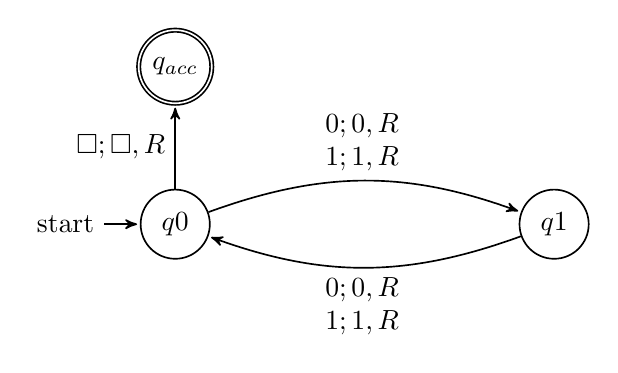
\begin{tikzpicture}[->,>=stealth',shorten >=1pt, auto, node distance=2cm, semithick]
        \tikzstyle{every state}=[text=black, fill=none]
        
        \node[initial,state] (q0)          {$q0$};
        \node[state]         (q1) [right of=q0, xshift=80pt] {$q1$};
        \node[state,accepting]   (qacc) [above of=q0] {$q_{acc}$};
        
        \path (q0) edge [bend left=20] node {\parbox{1cm}{$0; 0,R$\newline $1; 1, R$}} (q1)
            (q1) edge [bend left=20] node {\parbox{1cm}{$0; 0,R$\newline $1; 1, R$}} (q0)
            (q0) edge  [bend left=0] node {$\square; \square, R$} (qacc)
        ;
    \end{tikzpicture}
    &
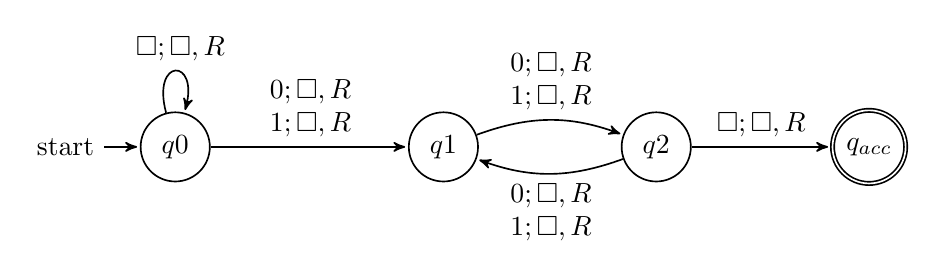
\begin{tikzpicture}[->,>=stealth',shorten >=1pt, auto, node distance=2cm, semithick]
        \tikzstyle{every state}=[text=black, fill=none]
        
        \node[initial,state] (q0)          {$q0$};
        \node[state]         (q1) [right of=q0, xshift=40pt] {$q1$};
        \node[state]         (q2) [right of=q1, xshift=20pt] {$q2$};
        \node[state,accepting]   (qacc) [right of=q2, xshift=20pt] {$q_{acc}$};
        
        \path (q0) edge [loop above] node {\parbox{1cm}{$\square; \square, R$}} (q0)
        (q0) edge [bend left=00] node {\parbox{1cm}{$0; \square,R$\newline $1; \square, R$}} (q1)
            (q1) edge [bend left=20] node {\parbox{1cm}{$0; \square,R$\newline $1; \square, R$}} (q2)
            (q2) edge [bend left=20] node {\parbox{1cm}{$0; \square,R$\newline $1; \square, R$}} (q1)
            (q2) edge  [bend left=0] node {$\square; \square, R$} (qacc)
        ;
    \end{tikzpicture}
    
    \end{tabular}
    
    Example strings in $A_{TM}$
    
    \vfill
    
    Example strings in  $E_{TM}$
    
    \vfill
    
    Example strings in  $EQ_{TM}$
    
    \vfill
    
    \newpage
    
    {\bf  Theorem}: $A_{TM}$  is  Turing-recognizable.
    
    
    {\bf  Strategy}:  To prove this theorem, we need  to  define  a Turing  machine  $R_{ATM}$ such that 
    $L(R_{ATM}) = A_{TM}$.
    
    
    Define $R_{ATM} =  $ ``
    
    \vspace{150pt}
    
    
    Proof of correctness: 
    
    
    \vfill
    \vfill
    
    We will show that $A_{TM}$ is undecidable.   {\it First, let's explore what that means.}
    
    \newpage
    
    To prove that a computational problem is {\bf decidable}, we find/ build a Turing 
    machine that recognizes the language encoding the computational problem, and that 
    is a decider.
    
    
    How do we prove a specific problem is {\bf not decidable}?
    
    How would we even find such a computational problem?
    
    
    {\it Counting arguments for the existence of an undecidable language:}
    \begin{itemize}
        \item The set of all Turing machines is countably infinite.
        \item Each recognizable language has at least one Turing machine that recognizes it (by definition), 
        so there can be no more Turing-recognizable
        languages than there are Turing machines. 
        \item Since there are infinitely many Turing-recognizable languages
        (think of the singleton sets), there are countably infinitely 
        many Turing-recognizable languages.
        \item Such the set of Turing-decidable languages is an infinite subset 
        of the set of Turing-recognizable languages, the set of 
        Turing-decidable languages is also countably infinite.
    \end{itemize}
    
    Since there are uncountably many languages (because $\mathcal{P}(\Sigma^*)$
    is uncountable), there are uncountably many unrecognizable languages
    and there are uncountably many undecidable languages.
    
    
    Thus, there's at least one undecidable language!
    
    \vfill
    
    {\bf What's a specific example of a language that is unrecognizable or undecidable?}
    
    To prove that a language is undecidable, we need to prove that there is no Turing machine that decides it.
    
    {\bf Key idea}: proof by contradiction relying on self-referential disagreement.
    
    

{\bf  Theorem}: $A_{TM}$  is  not  Turing-decidable.

{\bf  Proof}: Suppose {\bf towards a  contradiction}  that there  is a Turing machine  that decides $A_{TM}$.  
We call this presumed machine  $M_{ATM}$.

By  assumption, for every  Turing machine  $M$ and every  string $w$

\begin{itemize}
\item If $w \in L(M)$, then  the computation of $M_{ATM}$  on  $\langle M,w \rangle ~~ \underline{\phantom{\hspace{2.5in}}}$
\item If $w \notin L(M)$, then  the computation of $M_{ATM}$  on  $\langle M,w \rangle ~~ \underline{\phantom{\hspace{2.5in}}}$
\end{itemize}


Define  a {\bf new} Turing machine using  the high-level description:
\begin{quote}
$D =  $`` On  input $\langle M \rangle$, where  $M$  is  a Turing machine:
\begin{itemize}
\item[1.] Run  $M_{ATM}$ on  $\langle M, \langle M \rangle  \rangle$.
\item[2.] If $M_{ATM}$ accepts, reject; if  $M_{ATM}$ rejects, accept."
\end{itemize}
\end{quote}


Is $D$ a  Turing machine?

\vspace{30pt}

Is  $D$ a  decider? 

\vspace{30pt}

What is the result of the computation  of $D$  on  $\langle D \rangle$?

\vfill


\newpage

{\bf Summarizing}: 

\begin{itemize}
    \item $A_{TM}$  is recognizable.
    \item $A_{TM}$  is  not  decidable.
\end{itemize}

\vfill

Recall definition: A language $L$ over an  alphabet $\Sigma$ is called {\bf co-recognizable} if its complement,  defined
as $\Sigma^* \setminus L  = \{ x  \in  \Sigma^* \mid x \notin  L \}$, is Turing-recognizable.

and Recall  Theorem (Sipser Theorem 4.22): A  language is Turing-decidable if and only if both  it and its complement
are Turing-recognizable.

\vfill

\begin{itemize}
    \item $A_{TM}$  is recognizable.
    \item $A_{TM}$  is  not  decidable.
    \item $\overline{A_{TM}}$   is  not  recognizable.
    \item $\overline{A_{TM}}$   is  not  decidable.
\end{itemize}

\vfill \vfill
\section*{Week8 wednesday}


{\bf Mapping reduction}

Motivation: Proving that $A_{TM}$ is undecidable was hard. How can we leverage that work? 
Can we relate the decidability / undecidability of one problem to another?

\begin{quote}
If problem $X$ is {\bf no harder than} problem $Y$

\ldots and if $Y$ is easy,

\ldots then $X$ must be easy too.
\end{quote}


\begin{quote}
    If problem $X$ is {\bf no harder than} problem $Y$
    
    \ldots and if $X$ is hard,
    
    \ldots then $Y$ must be hard too.
\end{quote}

``Problem $X$ is no harder than problem $Y$'' means 
``Can answer questions about membership in $X$ by converting them to questions about membership in $Y$''.



Definition:  $A$ is  {\bf  mapping  reducible to} $B$  means there is a computable function 
$f : \Sigma^* \to \Sigma^*$ such that {\it for all} strings  $x$ in $\Sigma^*$, 
\[
x  \in  A \qquad \qquad \text{if and  only  if} \qquad \qquad f(x) \in B.
\]
Notation:  when $A$  is mapping reducible to $B$, we write $A  \leq_m B$.

{\it Intuition:} $A \leq_m B$ means $A$ is no harder than $B$, i.e. that the level 
of difficulty of $A$ is less than or equal the level of difficulty of $B$.

\vfill

{\bf TODO} 
\begin{enumerate}
\item What is a computable function?
\item How do mapping reductions help establish the computational difficulty of languages?
\end{enumerate}

\newpage
{\bf Computable functions}

Definition: A function $f: \Sigma^* \to \Sigma^*$ is a {\bf computable function} means there is some Turing machine such that, 
for each $x$, on input $x$ the Turing machine halts with exactly $f(x)$ followed by all blanks on the tape

\vspace{50pt}


{\it Examples of computable functions}:

The function that maps a string to a string which is one character longer and 
whose value, when interpreted as a fixed-width binary representation of a
nonnegative integer is twice the value of the input string (when interpreted as 
a fixed-width binary representation of a non-negative integer)
\[
f_1: \Sigma^* \to \Sigma^* \qquad  f_1(x)  = x0
\]

To prove $f_1$ is computable function, we define a Turing machine computing it.

{\it High-level description}
\begin{quote}
    ``On input $w$
    
    1. Append $0$ to $w$.
    
    2. Halt.''
\end{quote}

{\it Implementation-level description}
\begin{quote}
    ``On input $w$
    
    1. Sweep read-write head to the right until find first blank cell.
    
    2. Write 0.
    
    3. Halt.''
\end{quote}

{\it Formal definition} $(\{q0, qacc, qrej\}, \{0,1\}, \{0,1,\textvisiblespace\},\delta, q0, qacc, qrej)$
where $\delta$ is specified by the state diagram: 


\newpage


The function that maps a string to the result of repeating the string twice.
\[
f_2: \Sigma^* \to \Sigma^* \qquad f_2( x )  =  xx
\]

\vfill


The function that maps strings that are not the codes of NFAs to the empty 
string and that maps strings that code NFAs to the code of a DFA that recognizes
the language recognized by the NFA produced by the macro-state construction from Chapter 1.


\vfill


The function that maps strings that are not the codes of Turing machines to the empty 
string and that maps strings that code Turing machines to the code of the 
related Turing machine that acts like the Turing machine coded by the input, except
that if this Turing machine coded by the input tries to reject, the 
new machine will go into a loop.
\[
f_4: \Sigma^* \to \Sigma^*  \qquad f_4( x )  =   \begin{cases}  \varepsilon \qquad&\text{if $x$ is not the code of  a TM} \\
\langle (Q \cup \{q_{trap} \}, \Sigma, \Gamma, \delta', q_0, q_{acc}, q_{rej} ) \rangle \qquad&\text{if $x = \langle (Q, \Sigma, \Gamma, \delta, q_0, q_{acc}, q_{rej} )\rangle$}\end{cases}
\]
where $q_{trap} \notin Q$ and 
\[\delta'( (q,x) ) = \begin{cases}
(r,y,d) &\text{if $q \in Q$, $x \in \Gamma$, $\delta ((q,x)) = (r,y,d)$, and  $r \neq  q_{rej}$} \\
(q_{trap}, \textvisiblespace, R) & \text{otherwise}
\end{cases}
\]
\vfill
\vfill

\newpage

Definition:  $A$ is  {\bf  mapping  reducible to} $B$  means there is a computable function 
$f : \Sigma^* \to \Sigma^*$ such that {\it for all} strings  $x$ in $\Sigma^*$, 
\[
x  \in  A \qquad \qquad \text{if and  only  if} \qquad \qquad f(x) \in B.
\]

{\it Making intutition precise \ldots}

{\bf Theorem} (Sipser 5.22): If $A \leq_m B$ and $B$ is decidable, then $A$ is decidable.
    
\vfill


{\bf Theorem} (Sipser 5.23): If $A \leq_m B$ and $A$ is undecidable, then $B$ is undecidable.
    
\vfill
 \vfill
\section*{Week8 friday}



Recall definition:  $A$ is  {\bf  mapping  reducible to} $B$  means there is a computable function 
$f : \Sigma^* \to \Sigma^*$ such that {\it for all} strings  $x$ in $\Sigma^*$, 
\[
x  \in  A \qquad \qquad \text{if and  only  if} \qquad \qquad f(x) \in B.
\]
Notation:  when $A$  is mapping reducible to $B$, we write $A  \leq_m B$.

{\it Intuition:} $A \leq_m B$ means $A$ is no harder than $B$, i.e. that the level 
of difficulty of $A$ is less than or equal the level of difficulty of $B$.


{\it Example}: $A_{TM} \leq_m A_{TM}$ 

\vfill

{\it Example}: $A_{DFA} \leq_m \{ ww \mid  w \in \{0,1\}^* \}$ 

\vfill






\newpage

    {\bf Halting problem}
    \[
    HALT_{TM} = \{ \langle M, w \rangle \mid \text{$M$ is a  Turing machine, $w$ is  a string, and $M$ halts on $w$} \}
    \]
    
    Define $F: \Sigma^* \to \Sigma^*$ by
    \[
    F(x) =  \begin{cases}
    const_{out} \qquad &\text{if  $x \neq \langle M,w \rangle$ for any Turing machine  $M$ and string  $w$ over the alphabet of $M$} \\
    \langle M', w \rangle \qquad &  \text{if $x = \langle M, w \rangle$ for some Turing machine  $M$ and string $w$ over the alphabet of $M$.}
    \end{cases}
    \]
    where $const_{out}  =  \langle  \includegraphics[width=1.5in]{../../resources/machines/Lect22TM1.png} ,  \varepsilon  \rangle$
    and  $M'$ is a Turing machine that computes like $M$ except, if the computation ever were to go to a  reject state,
    $M'$ loops instead.   


    $F( \langle \includegraphics[width=2.5in]{../../resources/machines/Lect22TM2.png} ,  \varepsilon  \rangle)$ =

    To use this function  to prove that $A_{TM} \leq_m HALT_{TM}$, we need  two claims:

    
    Claim (1): $F$ is computable \phantom{\hspace{2in}}
    
    \vfill

    Claim (2): for every  $x$,  $x \in  A_{TM}$ iff $F(x) \in HALT_{TM}$.  
    
    \vfill
    \vfill
    \vfill \vfill
\end{document}